\section{Auswertung}
\label{sec:Auswertung}

\subsection{Bestimmung des Emissionsvermögens}
Das Emissionsvermögen der einzelnen Oberflächen wird bestimmt, in dem die Thermospannung als Funktion von $T^4 - T_0^4$ aufgetragen wird. Aus der Steigung der Ausgleichsgeraden lässt sich dann $\epsilon$ bestimmen. \\
Die gemessene Raumtemperatur beträgt
\begin{align*}
  T_0 = 294.26 \, \text{K} \ .
\end{align*}
Die Thermospannungen bei den Temperaturen sind in Tabelle \ref{tab:Daten} aufgeführt.
\begin{table}
  \centering
  \begin{tabular}{c c c c c}
    \toprule
    	& \multicolumn{1}{c}{weiß} & \multicolumn{1}{c}{messingfarben} &	\multicolumn{1}{c}{schwarz} & \multicolumn{1}{c}{glänzend} \\
    $T$ / K & $U_\text{1}$ / mV & $U_\text{2}$ / mV & $U_\text{3}$ / mV & $U_\text{4}$ / mV \\
    \midrule
      368.15	&  1.09	&  0.20	 & 1.13  & 0.084 \\
      363.15	&  1.04	&  0.17	 & 1.05  & 0.068 \\
      358.15	&  0.93	&  0.16	 & 0.94  & 0.061 \\
      353.15	&  0.84	&  0.14	 & 0.85  & 0.047 \\
      348.15	&  0.73	&  0.12	 & 0.75  & 0.050 \\
      343.15	&  0.65	&  0.11	 & 0.66  & 0.041 \\
      338.15	&  0.56 &  0.092 & 0.57  & 0.033 \\
      333.15	&  0.48	&  0.086 & 0.49  & 0.037 \\
      328.15	&  0.40	&  0.072 & 0.41  & 0.026 \\
      323.15	&  0.33	&  0.057 & 0.34  & 0.023 \\
      318.15	&  0.26	&  0.047 & 0.26  & 0.021 \\
      313.15	&  0.19	&  0.032 & 0.19  & 0.022 \\
      308.15	&  0.13	&  0.024 & 0.13  & 0.015 \\
    \bottomrule
  \end{tabular}
  \caption{Die Thermospannung bei verschiedenen Temperaturen}
  \label{tab:Daten}
\end{table}

Die Offsetspannung vor und nach dem Versuch ist in Tabelle \ref{tab:Offset} aufgeführt und wird zu $U_\text{0}$ gemittelt.

\begin{table}
  \centering
  \begin{tabular}{c c c}
    \toprule
      & $U_\text{vor}$ & $U_\text{nach}$  \\
      $U$ / mV      & 0.013 & 0.006       \\
      $U_\text{0}$  & 0.007 &             \\
    \bottomrule
  \end{tabular}
  \caption{Die gemittelte Offsetspannnung}
  \label{tab:Offset}
\end{table}

Mit den Tabellen \ref{tab:Daten} und \ref{tab:Offset}, sowie $T_0$ ergeben sich die Abbildungen \ref{fig:ThermoW} bis \ref{fig:ThermoG}.
\begin{figure}[H]
  \centering
  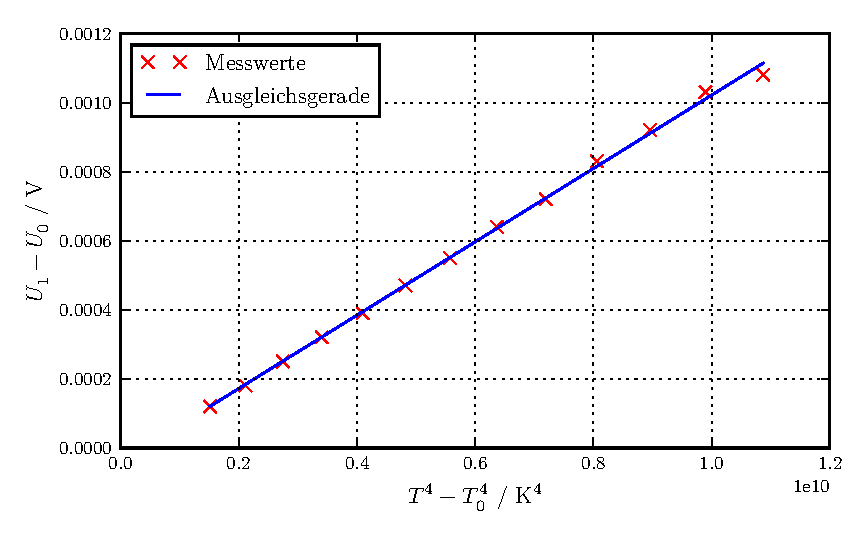
\includegraphics[width=\textwidth]{ThermoW.pdf}
  \caption{Ausgleichsgerade der Messwerte für die weiße Oberfläche}
  \label{fig:ThermoW}
\end{figure}

\begin{figure}[H]
  \centering
  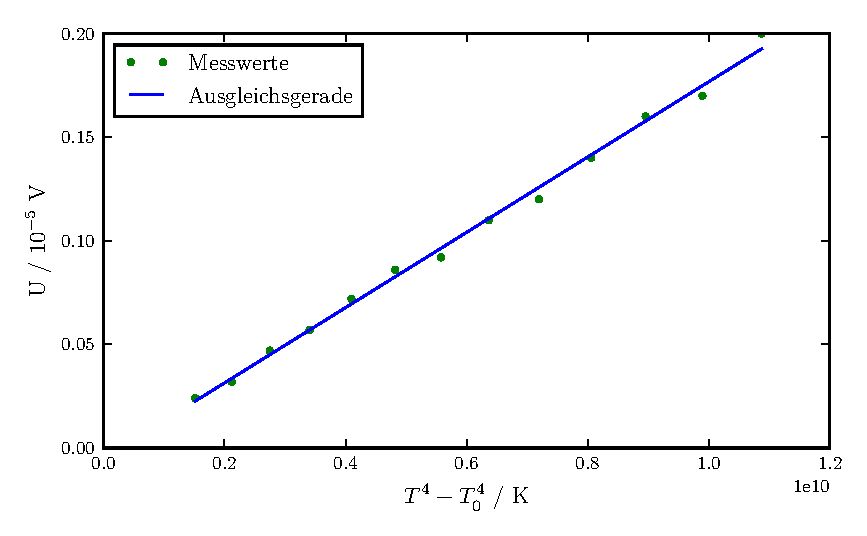
\includegraphics[width=\textwidth]{ThermoM.pdf}
  \caption{Ausgleichsgerade der Messwerte für die messingfarbene Oberfläche}
  \label{fig:ThermoM}
\end{figure}

\begin{figure}[H]
  \centering
  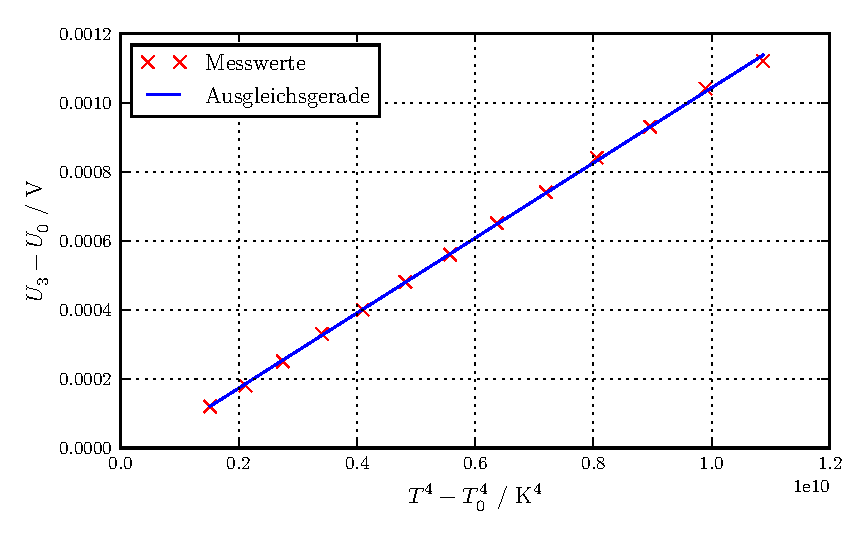
\includegraphics[width=\textwidth]{ThermoS.pdf}
  \caption{Ausgleichsgerade der Messwerte für die schwarze Oberfläche}
  \label{fig:ThermoS}
\end{figure}

\begin{figure}[H]
  \centering
  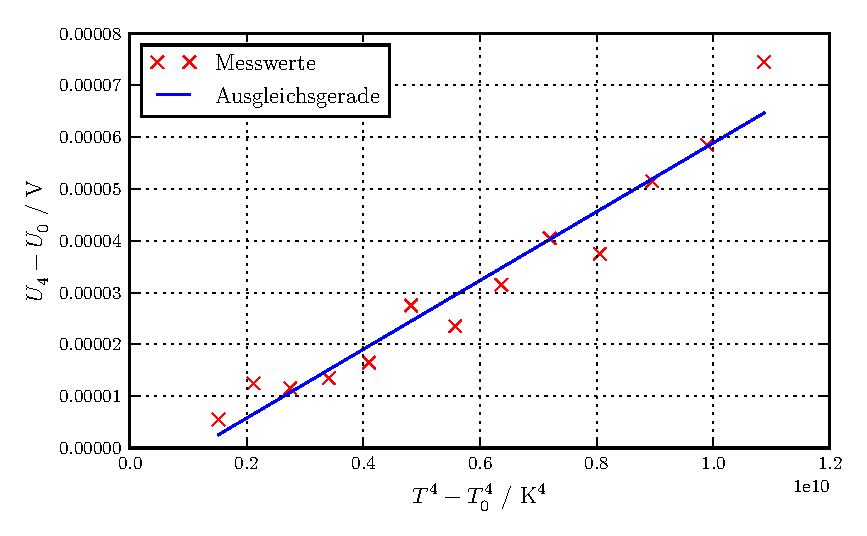
\includegraphics[width=\textwidth]{ThermoG.pdf}
  \caption{Ausgleichsgerade der Messwerte für die glänzende Oberfläche}
  \label{fig:ThermoG}
\end{figure}
Die Steigung und der Fehler der Ausgleichsgeraden werden mit der linearen Regression durch Python 3.4.3 ermittelt und sind im folgenden aufgelistet.
\begin{align*}
  m_\text{weiß}     &= (\num{10.6 +- 0.1})   \cdot 10^{-14} \, \text{V/K}^4 \\
  m_\text{messing}  &= (\num{1.82 +- 0.04})  \cdot 10^{-14} \, \text{V/K}^4 \\
  m_\text{schwarz}  &= (\num{10.87 +- 0.07}) \cdot 10^{-14} \, \text{V/K}^4 \\
  m_\text{glänzend} &= (\num{0.66 +- 0.05})  \cdot 10^{-14} \, \text{V/K}^4 \\
\end{align*}
Mit der Annahme, dass die schwarze Oberfläche ein Schwarzer Körper ist($\epsilon_\text{schwarz} = 1$), folgt mit der Gleichung \ref{eqn:epsilon}, für die anderen Oberflächen ein Emissionsvermögen von:
\begin{equation}
  \epsilon_\text{i} = \frac{m_\text{i}}{m_\text{schwarz}}
  \label{eqn:epsilon}
\end{equation}
\begin{align*}
  \epsilon_\text{schwarz}  \, &= (\num{1.0 +- 0.0})     \\
  \epsilon_\text{weiß}     \, &= (\num{0.98 +- 0.01})   \\
  \epsilon_\text{messing}  \, &= (\num{0.167 +- 0.004}) \\
  \epsilon_\text{glänzend} \, &= (\num{0.061 +- 0.004}) \\
\end{align*}
Die Fehlerformel von $\varepsilon_\text{i}$ folgt mit Formel \ref{eqn:var} zu:
\begin{equation}
  \Delta \varepsilon_\text{i} = \frac{\Delta m_\text{i}}{m_\text{schwarz}} \ .
\end{equation}

\subsection{Thermospannunng im Verhältnis zum Abstand}
Die Thermospannung der weißen Oberfläche gegen $\frac{1}{A^2}$ aufgetragen ergibt Abbildung \ref{fig:Abstand}. Die dazu gehörigen Messwerte sind in Tabelle \ref{tab:Abstand} aufgelistet.
\begin{table}[H]
  \centering
  \begin{tabular}{c c c}
      A / m & $\frac{1}{A^2}$ / $\frac{1}{\text{m}^2}$ & $U_\text{weiß}$ / mV \\
    \midrule
      0.100  & 100.0 & 0.247 \\
      0.125	& 64.0   & 0.238 \\
      0.150	& 44.4   & 0.228 \\
      0.175	& 32.7   & 0.217 \\
      0.200	& 25.0   & 0.202 \\
      0.225	& 19.8   & 0.189 \\
      0.250	& 16.0   & 0.177 \\
      0.275	& 13.2   & 0.162 \\
      0.300	& 11.1   & 0.149 \\
      0.325	& 9.5    & 0.137 \\
      0.350	& 8.2    & 0.128 \\
  \end{tabular}
  \caption{Messergebnisse für das Verhältnis zwischen Thermospannung und $\frac{1}{A^2}$}
  \label{tab:Abstand}
\end{table}

\begin{figure}[H]
  \centering
  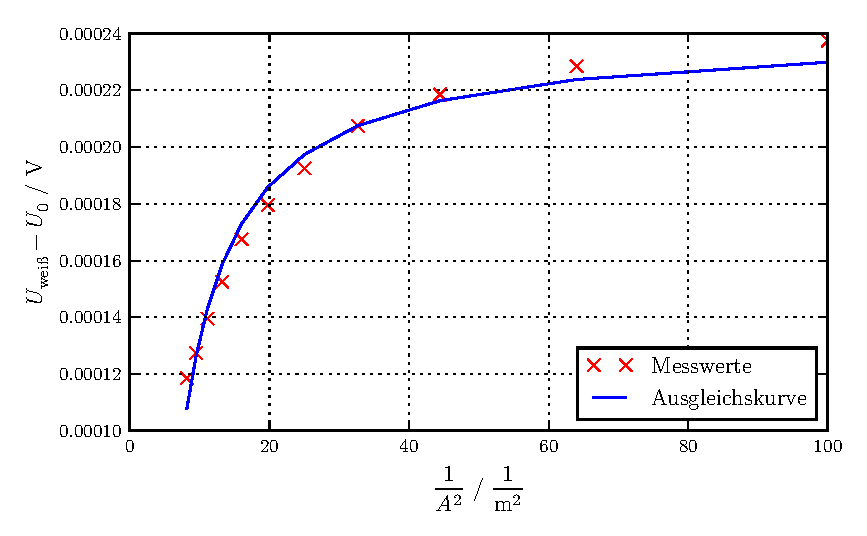
\includegraphics[width=\textwidth]{ThermoAbstand.pdf}
  \caption{Graph für das Verhältnis zwischen Thermospannung und $\frac{1}{A^2}$}
  \label{fig:Abstand}
\end{figure}
In Abbildung \ref{tab:Abstand} wird deutlich, dass die Ausgleichskurve folgender Funktion entspricht:
\begin{equation}
  y = \frac{a}{x^2} + b \ .
\end{equation}
Die Parameter $a$ und $b$ der Funktion werden mit Python 3.4.3 berechnet.
\begin{align}
  a &= (\num{-1.09 +- 0.05}) \cdot 10^{-3} \, \frac{\text{V}}{\text{m}^2} \\
  b &= (\num{2.41 +- 0.04}) \cdot 10^{-4} \, \text{V}
\end{align}
